\chapter{State of the Art}
\label{ch:StateOfTheArt}
In this chapter, we further explain the theory of reactive programming and approaches in debugging applications that use this pattern. We also examine existing debugging tools that target reactive programming frameworks and libraries as well as reactive programming libraries for JavaScript (JS). We discuss the Chrome Reactive Inspector (CRI) and work targeting CRI prior to this thesis in detail in addition to its main competitor RxFiddle.

\section{Implementation of reactive systems}
Although there are many implementations of reactive systems for a multitude of programming languages, most of them are designed similarly and share the same building blocks. This section introduces (functional) reactive programming in general, and later the JavaScript libraries RxJS and BaconJS as specific implementations of the paradigm in detail. We also point out the main differences between the two libraries, their history, and their relevance by examining some statistics of the respective source code repositories hosted on GitHub \cite{RxJSRepo} \cite{BaconJSRepo}.

	\subsection{Reactive programming}
	A reactive programming framework or library removes a lot of boilerplate code the developer usually has to implement to propagate changes and events throughout a software system. It advances the well known Observer Design Pattern and overcomes several shortcomings of that approach. In the Observer Design Pattern, a \emph{subject} propagates changes to its state to a list of previously registered observers \cite{FRP}. A \emph{subject} only returns one value, i.e. its state, while an \emph{observable} (also called \emph{behavior}) in reactive programming can provide multiple values over time as a stream.
	In addition to \emph{observables}, which provide varying values over time, a reactive programming implementation usually includes a construct called \emph{events} or \emph{event streams} \cite{BaconJS}, which handles discrete events over time.
	
	What we refer to as an \emph{observable} actually consists of three parts - a \emph{producer} that produces values over time, the actual \emph{observable} that stores these values, and the \emph{observer} that notifies all \emph{subscribers} (sometimes also called \emph{consumers}). The notification of the \emph{subscribers} is specific to \emph{push-based} systems where the values are pushed through the reactive system when a new value arrives. This stands in contrast to a pull-based system in which values are only pulled on demand when they are requested by a \emph{subscriber} of an \emph{observable} or any of its descendants (i.e. other \emph{observables} that depend upon it).
	\emph{Observables} are categorized as either \emph{hot} or \emph{cold} \cite{HotVsCold}. A \emph{cold} \emph{observable} will create a new \emph{producer} each time a \emph{subscriber} subscribes to its \emph{observer}. The \emph{producer} will be destroyed once the \emph{subscriber} unsubscribes, i.e. the resources it uses are freed and it signals its own termination. This is referred to as the unicast approach. All \emph{subscribers} to a \emph{hot} \emph{observable}, on the other hand, will (usually) share one \emph{producer}. This is referred to as the multicast approach.
	
	The reactive programming paradigm is declarative in its nature. This limits side-effects and is usually implemented with many \emph{pure} functions, which serve as \emph{operators}, that are used to transform, combine or change behavior of \emph{observables} and \emph{event streams}. The \emph{operators} return a new \emph{observable} that depends upon the \emph{observable} on which the \emph{operator} was used. Using these operators, the developer declares dependencies between observables, which creates more comprehensible program code and structure \cite[Why Reactive Programming?]{ReactiveInspector} than imperative programming style would produce.

	\subsection{RxJS and BaconJS}
	AThere are many JavaScript implementations of the reactive programming paradigm such as Cycle \cite{CycleJS}, Kefir \cite{KefirJS} or Most \cite{MostJS}. An extensive and maintained list of reactive frameworks and libraries for JavaScript can be found at \cite{FRPJSList}. This section is focused on ReactiveX for JavaScript (RxJS) \cite{RxJS} and Bacon (BaconJS) \cite{BaconJS} because these are the libraries the Chrome Reactive Inspector currently supports.
	
	\textbf{Rx.js}\\
	Reactive Extensions for JavaScript or RxJS \cite{RxJS} is the JavaScript implementation of ReactiveX. ReactiveX implementations also exist for a number of other programming languages, such as, Java (RxJava), Scala(RxScala) or C\#(Rx.NET). In extension to the basic concepts of reactive programming, RxJS implements \emph{subjects} and \emph{schedulers}. A \emph{subject} represents the implementation of an \emph{event stream} and is the only option to realize a multicast \emph{observable}, since \emph{observables} are \emph{cold} \emph{observables} in RxJS. \emph{Subjects} can be both \emph{observer} and \emph{observable} at the same time. To convert a \emph{cold} \emph{observable} into a \emph{hot} one, the functions \emph{share} or \emph{publish} can be used. They use a \emph{subject} internally to track the shared \emph{producer}. A \emph{subject} will be terminated once the last \emph{subscriber} unsubscribes. \emph{Schedulers} are centralized dispatchers which are used to control concurrency and allow influencing the scheduling behavior when asynchronous functions such as \emph{setTimeout}\cite{RxJsDocu} are called. \emph{Observers} raise special events if the \emph{observable} is completed or reaches an error state. The \emph{observable} will not be reusable afterwards, even if it is a \emph{subject}, which is a main difference to the later discussed BaconJS. RxJS provides several utility functions to convert values, arrays or events into observables \cite{ThesisBaradur}. A basic example of RxJS code to show the general structure can be seen in listing \ref{lst:Rx} (Source: \cite{RxJsDocu} under manual/overview.html).
	The latest stable version of RxJS is version 5.5.6 with version 6.0.0-alpha already under active development. RxJS is licensed under the Apache 2.0 license and the source code is publicly available on GitHub \cite{RxJSRepo}.

	\begin{lstlisting}[language=JavaScript, caption={Example of RxJS code.},label={lst:Rx}]
	var button = document.querySelector('button');
	Rx.Observable.fromEvent(button, 'click')
	.throttleTime(1000)
	.scan(count => count + 1, 0)
	.subscribe(count => console.log(`Clicked ${count} times`));
	\end{lstlisting}
	
	\textbf{Bacon.js}\\
	The basic concepts of BaconJS \cite{BaconJS} are \emph{properties} - which represent the \emph{observables} - and \emph{event streams} that handle distinct events. 
	In contrast to RxJS, BaconJS's \emph{properties} are always \emph{hot} \emph{observables}. In addition, an error in an \emph{event stream} or \emph{property} will not cause them to terminate. Errors are, therefore, handled as any other value, which provides more fine-grained control for the developer. However, the \emph{endOnError} function can be used if the termination is desired. 
	Another advantage of BaconJS is the \emph{spy} function, which can be used to observe the internal workings and, therefore, greatly reduces the required effort to create complementary tooling like CRI or RxFiddle. It can also be used to easily create extensive logging without modifying the rest of the reactive application source code. According to the author(s), BaconJS was developed because they got frustrated with RxJS as its source code was not publicly available at the time and the documentation was minimal. They also claim that BaconJS has a more consistent and glitch-free stream/property behavior \cite{BaconJSRepo}. However, they explain that RxJS has less overhead and consequently a better performance. 
		\begin{lstlisting}[language=JavaScript, caption={Example of BaconJS code.},label={lst:Bacon}]
	$("#username input").asEventStream("keyup")
	.map(function(event) {
	return $(event.target).val();
	})
	.toProperty("")
	\end{lstlisting}
	BaconJS is still under active development, with the latest stable version being 2.0.0. It is licensed under the MIT license and the source code is publicly available on GitHub \cite{BaconJSRepo}.

	While BaconJS is a newer reactive programming library and was developed to handle some shortcomings of RxJS, according to the GitHub statistics RxJS has still a much larger community. RxJS has 387 watches, 10540 stars, 991 forks and 185 contributors for the currently active repository, while BaconJS has 156 watches, 5839 stars, 328 forks and 83 contributors in total (last accessed: 31.1.2018 18:22).
	In addition, since RxJS was started earlier and due to its similarity to ReactiveX implementations in other languages, a number of tools and utility libraries exist exclusively for RxJS - including RxFiddle.

\subsection{Debugging Reactive Code}
Debugging is an important part of any form of programming. Virtually all of the most commonly used IDEs offer a precise detection of lexical and syntactic errors, such as misspelled keywords or missing control characters. They further apply the concept of breakpoints, are probably the most useful feature for in-depth code and state inspection at a precise point during the application's execution. In addition to simple breakpoints, modern IDEs also support conditional breakpoints, step by step execution, event logging, stack trace inspection and many other tools to debug code at runtime. Due to the declarative nature of  reactive programming, traditional breakpoints and similar runtime debugging features cannot be used as easily as with imperative programming. For some IDEs the most basic form of declarative programming, chained function calls (also called Method chaining \cite{MethodChaining}), provide an obstacle for a user because the IDE's breakpoints are line- and not character-position-based. But even if the IDE can handle breakpoints inside anonymous functions for the usual navigation features like \emph{Step Over} and \emph{Step Into}, it is not trivial to balance between providing the necessary fine-grained stepping and having too many steps for the developer to iterate. For example one of the most advanced IDEs there is, Visual Studio (2017) for .NET, will step over the whole batch of chained functions if the developer uses \emph{Step Over}, but will step into the first anonymous function in the chain if the developer uses \emph{Step Into}. The developer can then use \emph{Step Over} to enumerate the anonymous functions passed to the chained functions (see listing \ref{lst:CSharp_LINQ}). This is a very specialized and desirable behavior that will match the intent of the developer most times when using the .Net Framework built-in \emph{.NET Language-Integrated Query Expressions} (LINQ), but this behavior will break as soon as a custom function is added to the chain (\emph{DoCustom} in the code example). Now the \emph{Step Into} on line 1 will step into \emph{DoCustom} for each entry in the list and will then step out of the batch of chained functions to line 10. If a similar code example in BaconJS is debugged with the step-by-step debugging feature of Google Chrome, it will actually step through the BaconJS library code even if the developer just uses \emph{Step Over}. As BaconJS or other reactive programming libraries are not part of native JavaScript, Google Chrome has no means to determine if the user wants to step through the library code or not.
This example shows that debugging declarative code is still a hard task for modern IDEs, especially if Out-of-Order execution (LINQ Expressions are executed Out-of-Order) is added. The IDE cannot always correctly interpret the developer's intentions when debugging declarative code with step-by-step execution. The developer might want to debug the custom chained function or they might want to iterate the anonymous functions passed as arguments (like "s => s.ToUpper()" line 2 and "s => s" line 8 in listing \ref{lst:CSharp_LINQ}) to the chained functions. They might also want to step through framework functions such as \emph{Select}, \emph{Where}, or \emph{OrderBy} in .NET themselves, which is made possible by the framework debugging option in Visual Studio 2017. 
For big collections or, in the case of reactive programming, observables with many submitted values, this problem is also increased if there are too many single executions of one or more anonymous functions for the developer to step through. Another example for this is a breakpoint inside an anonymous function that is passed to a declarative function (like\emph{Where} in C\# or \emph{map} in BaconJS), which halts the application for each element in the collection or data stream.

%TODO: language is c# but the compilation would not complete with "[Sharp]C" as language.
\begin{lstlisting}[language=JavaScript, caption={Simple example of .NET LINQ in C\# to show the steps the Visual Studio 2017 for .NET debugger takes while debugging step-by-step.},label={lst:CSharp_LINQ}]
 var lst = new List<string>{"test1","test2"};
 var result = lst.Select(s => s.ToUpper())
 .Where(s =>
 {
	var b = s.StartsWith("t");
	return !b && s.StartsWith("T");
 })
.OrderBy(s => s)
.DoCustom()
.ToList();
\end{lstlisting}

This shows that a traditional debugger is not suitable for the use with declarative programming in general and reactive programming in particular. While the Visual Studio debugger is still somewhat useful to debug LINQ in .Net, because multiple specialized behaviors have been implemented over the years and LINQ expressions will most likely not cover the entire application and are often used to execute short tasks inside an imperative program flow, observables in a reactive application are usually much more intertwined and make up the general flow of the program; making a traditional debugger more of an obstacle.

As described in \cite{MSDN_DebugginObservables} reverting to the most basic debugging technique sometimes called \emph{printf-debugging} (or in the RxJS terms \emph{do-debugging}), to generate debug outputs or traces by directly modifying the source code, generally provides better results than using advanced features of a traditional debugger. Some shortcomings of this basic technique can be mitigated by using sophisticated tools like shown in \cite{ShinyGraphFromLog} in the section "The Reactive Log" where the log of an application is visualized in a dependency graph containing code pieces as nodes. Do-debugging still requires modification of the original source code to trace the programs execution path and pollutes it with statements that do not contribute to the program logic itself, making the code harder to read. \cite{PaperReactiveProgramming} describe the main issue to be missing abstractions and a "mismatch in the mental model", because traditional debuggers operate mainly on the runtime stack information and "do not consider any other abstraction within the running code" \cite{ThesisAbbas}. Traditional debuggers, therefore, make it very hard for the developer to detect flaws in dependencies between reactive entities.

In the programming language JavaScript (JS) it is, unlike in compiled languages, by design harder to detect errors in the written code, because it is an interpreted script language and the JS code is not compiled before execution. The general advantage of a script language being able to change the code at runtime and omitting the computation time needed to compile an application, is shadowed by the fact that many bugs can only be found at runtime as well. In addition, Type-safe languages can detect many errors even before compilation by verifying that the used types are compatible. This makes reactive applications written in JavaScript even harder to debug than their counterparts in other languages.

Currently, there are few tools to help the developer debug reactive applications and apart from RxFiddle (described in detail in section \ref{sec:RxFiddle}) none of them, as far as we known, support debugging reactive JavaScript applications. One of those tools is \cite{ShinyGraphFromLog} as mentioned above. Another is the Reactive Inspector for the Scala language \cite{ReactiveInspector} started and maintained by Prof. Dr. Guido Salvaneschi working in the Software Technology Group of the Technical University of Darmstadt, Germany.
The Reactive Inspector is an extension of the Scala IDE for Eclipse. Many features and the basic concepts that are implemented in the \emph{Chrome Reactive Inspector(CRI)} originate from the Reactive Inspector. This includes the representation of observables and their dependencies in a dependency graph called \emph{reactive tree}, the option to query the history of this graph, or the option to search for a specific node in the current graph. They are described in details in section \ref{sec:PreviousCRI}. One main feature of the Reactive Inspector which is currently not implemented for the CRI is called \emph{Tree Outline}. Here the user can quickly jump to different areas of the dependency graph. This is useful for applications with large graphs.

\section{Previous work on the CRI and its main competitor}
In this section, we will cover the previous work on the Chrome Reactive Inspector (CRI) as well as RxFiddle which is the main competitor for the CRI because both have a similar goal to help developers debug reactive systems in JavaScript with abstract concepts that go beyond traditional debugging.

	\subsection{The Chrome Reactive Inspector}
	\label{sec:PreviousCRI}
	The Chrome Reactive Inspector is based on the Reactive Inspector for Scala \cite{ReactiveInspector} and was developed by the Software Technology Group at the TU-Darmstadt Germany supervised by Prof. Dr. Guido Salvaneschi. It is implemented as a Google Chrome(Chrome) extension that extends the Chrome Developer Tools (DevTools) with another panel that inspects and instruments a target reactive Web application that is using RxJS or BaconJS. Prior to this thesis there have already been two Master theses targeting the CRI that provide the base theory and source code of this thesis.\\
	
	\textbf{Master Thesis by Waqas Abbas}\\
	
	\cite{ThesisAbbas} The main goal of the Master Thesis by Waqas Abbas was to develop and implement a concept for a Chrome extension based on the Reactive Inspector to debug reactive Web applications in JavaScript. One major difficulty was to find a viable solution for intercepting calls to the reactive libraries in order to retrieve the necessary information about observables and their dependencies that are used to build a dependency graph (called dependency tree in \cite{ReactiveInspector}) as well as to gather additional details like the variable name that directly correspond to observables and providing them with context by instrumenting the source code. An in-browser solution taken from a demo page \cite{JalangiDemo} of Jalangi was used to instrument and analyze the source code directly. The main Jalangi framework \cite{Jalangi} is currently not usable solely within a browser.
	Abbas also implemented several features to help the developer navigate and examine the dependency graph and its history. In this first version of the CRI, the user could already submit history queries that search the history of the graph for specific nodes or events like node creation, update or the creation of a dependency. In addition, the user could add \emph{reactive breakpoints} - breakpoints that pause the program execution when a specific event occurs - or search for a node in a large dependency graph.
	At the time the CRI supported BaconJS\cite{BaconJS} and parts of RxJS\cite{RxJS}. Abbas also added the first batch of small Web applications that could be used as test applications to manually verify features of CRI.\\		
		
	\textbf{Master Thesis by Pradeep Baradur}\\
	 \cite{ThesisBaradur} The main goal of the Master Thesis by Pradeep Baradur was to add full support for RxJS to CRI, especially all \emph{operators} and \emph{subjects}. Since RxJS does not provide a uniform way to intercept all calls to the library like the BaconJS's \emph{spy} function, this is a hard problem. For the actual implementation details see \cite{ThesisBaradur} or the \emph{rx-interception.js} file in the current version of CRI. Baradur also reworked loading of CRI's content scripts and instrumentation to only occur once the CRI DevTools panel is opened for an inspected Web application. This reduces the load on the browser if CRI is not currently used. He also extended the search and history query features to allow searching for dependents or dependencies of a node. The focus of his thesis in comparison to Abbas's shifted from being mainly a proof of concept to advancing the CRI to be more reliable and ultimately being usable in a production environment. This included rearranging the UI to be more consistent and improving reliability in general as well as adding additional test applications.\\		
		
	\textbf{Merging previous efforts}\\
	Since Waqas Abbas and Pradeep Baradur's works on the CRI partly overlapped and where developed in separate repositories, uniting both works was the first task for the thesis. Due to being developed separately after Baradur's Thesis started, the repositories shared no common history and due to many refactorings and renames in both projects as they advanced, merging the code base was not possible with automated tools and had to be done manually. Tracing the correlation between different changes was not trivial - in part because both theses were focused on advancing the project and less on maintainability and modularization. For this thesis, we took the source code of Pradeep Baradur's Thesis as a base and added features that Waqas Abbas developed after Baradur's Thesis had started. The main reason for this is that Baradur removed many bugs and race conditions that happened in some rarer cases of code execution order, in his goal to make CRI more reliable, which were outside of the scope of Abbas's work.
		
	\subsubsection{Exceptional properties of the CRI implementation}
	\label{sec:CRISpecials}
	The special method that is used to intercept the loading of a Web application by dynamically reloading the JavaScripts to allow direct access and replace specified scripts with an instrumented version has several implications that break the usual \emph{isolated world} \cite{GoogleApiContentScripts} of Google Chrome extensions and their content scripts. The loading of the inspected HTML is stopped, the HTML file is scanned for references to JavaScript files that are then loaded and, on demand, instrumented. The scripts are then executed within the context of the content script that does the instrumentation. This is necessary so that both the inspected pages own scripts as well as the content scripts of CRI that are responsible for the recording of the inner workings of the used reactive system share the same RxJS or BaconJS instance. But this approach also has some downsides, for example, a global variable in one of the inspected pages scripts may also be used in a script of CRI could cause unforeseen errors - e.g. common libraries like jQuery \cite{jQuery} that provide global objects will cause version conflicts. This also implies a potential security risk, because a Chrome extension runs in a \emph{trusted} context and has access to many Chrome APIs (Application programming interfaces) that are not accessible from a normal Web application - the CRI could, therefore, be manipulated through shared global variables to execute malicious code by an inspected page.
	Another implication of this approach is that CRI has to filter all referenced JS files of the inspected page to exclude all RxJS or BaconJS scripts from the loading process to use its own versions. This will lead to errors if the versions do not match exactly.
	Dynamically loading the scripts that are referenced by the inspected pages HTML also cannot handle any module loader without special interception logic. As module loaders are widely used in modern Web applications and are even part of the ECMA6 \cite{ECMA6import} standard as the \emph{import} keyword, this currently imposes a significant limitation on the number of Web applications CRI can be used with. We provide more detail and discuss some of the possible options in chapter \ref{ch:Future}.
	
	
	In addition to the special circumstances due to the dynamically loading of scripts in the shared context, CRI also uses a Demo \cite{JalangiDemo} in-browser version of the Jalangi \cite{Jalangi} that does not provide the full features of Jalangi. Instead, it only contains features used in the Demo - for example, the source code position information of functions and variables do not contain the scripts file name. Jalangi itself contains hundreds of analysis customization options that are not included in the in-browser Demo. Another obstacle presented by using the in-browser Demo script is that it is only available in the \emph{minified} version that is hard to read and debug.
	%TODO check all cite if it was compiled correctly
	
	\subsection{RxFiddle}
	\label{sec:RxFiddle}
	RxFiddle \cite{RxFiddle} is a tool developed as part of a Master Thesis by Herman Banken at the Delft University of Technology that displays interactive marble diagrams for RxJS Web applications. RxFiddle instruments the used RxJS library to collect information about the inner workings of the library. It is available as a Web application at \cite{RxFiddle} and the source code is publicly available at \cite{RxFiddleGitHub} under the MIT license. RxFiddle is the main competitor of CRI as it is the only other tool (that we are aware of) that tackles debugging for reactive systems in JavaScript. In RxFiddle the user can run JavaScript code visible on the left (1) and select a node from a simplistic dependency graph (2) to view a marble diagram showing details of its events, value streams (3), the interaction of operators and anonymous functions (4) passed to these operators.
	
	\begin{figure}[!h]
		\centering
		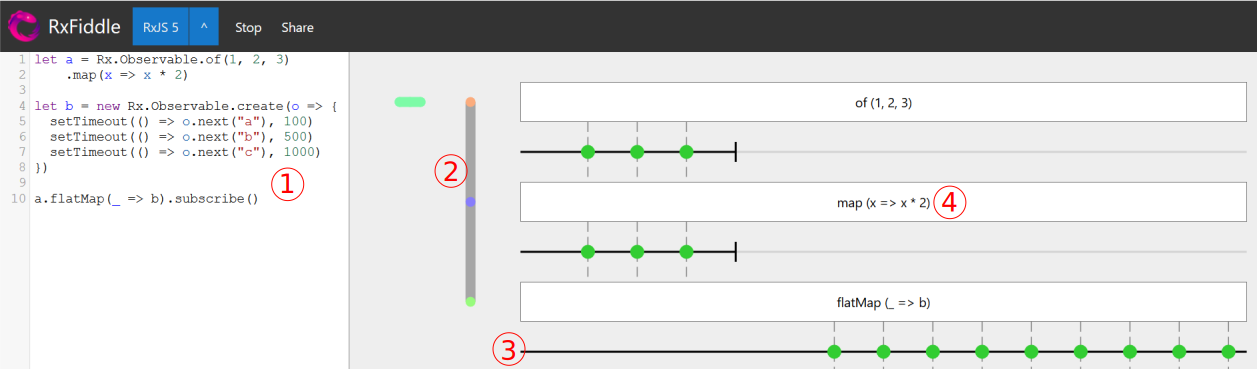
\includegraphics[scale=0.5,trim=0 0 0 0]{gfx/RxFiddleDemo.png}
		\caption{RxFiddle Demo \protect\cite{RxFiddle}}
		\label{fig:RxFiddleDemo}
	\end{figure}

	In the future, the author plans to support multiple additional collectors for RxScala, RxJava, RxSwift and/or RxNet \cite{RxFiddleTutorials}, which would record and transmit the necessary data on these platforms to RxFiddle. This would enable the user to use the same debugging environment which would be especially beneficial for applications that consist of a mixture of platforms e.g. a Web application with a RxJS front-end and RxNet back-end on the Web server.
	One of the limitations of RxFiddle is that there is no direct linking of the abstract representation to the actual source code like CRI provides with variable or method names if available for a node. This forces the developer to keep the reactive and declarative mindset but increases the time it takes to track down the responsible code that caused an issue that is detected in the abstract view. For example, the variables \emph{a} and \emph{b} do not appear anywhere in the abstract view (right side) of RxFiddle in figure \ref{fig:RxFiddleDemo}. The right side of the variable assignment of \emph{a} is present ("of(1, 2, 3)") and easy to find, but the assigned value to \emph{b} is listed as "Observable" which is hard to connect if multiple observables without direct dependencies exist. Although it has to be mentioned that CRI cannot handle multiple variables having the same variable name yet, even if they are in different scopes.
	RxFiddle also has trouble handling large applications properly according to the author \cite[Issue 6]{RxFiddleGitHub}. The data collection works fine - the tool is just not equipped to display and navigate large dependency graphs yet. Another limiting factor is the performance while rendering the graph or marble diagram. The author proposes several options to tackle this limitation like \emph{priority ranking}; for details see \cite[Issue 6]{RxFiddleGitHub}. Although displaying large applications in one graph is hard for CRI as well, RxFiddle requires more spaces of the User Interface (UI) for a single reactive operator and it currently has no option to zoom the graph of marble diagram. A large dependency graph for a single point in time used in CRI, where some descriptive details of the nodes are always visible, is easier to examine than a large marble diagram that shows all values over time as marbles, but only shows node information in tooltips that need to be opened first.
	A similar issue for RxFiddle is the displaying of rapidly updating observables like an observable created by the RxJS \emph{interval} function. Since each value update creates a new marble for the observable, the view becomes encumbered fast. As of this moment CRI also generates one or more steps for each update (if the node is not explicitly excluded). It is, however, still easily possible to examine node values in the first or last few steps of the history (jump to start or end and use the next/previous buttons). CRI can also query the result of a recording which provides means to cope with large dependency graphs or Histories. In RxFiddle the limiting factor for  fine-grained examination of nodes or values is the available space and the over-plotting of marbles. Details of nodes or marbles can only be viewed if the user is able to hover over them in order to open the tooltip. For a performance comparison between the newest version of CRI and RxFiddle regarding \emph{interval observables} see section \ref{sec:PerformanceEvaluation} since increasing the performance of CRI with this kind of observables was a goal of this thesis (discussed in section \ref{sec:RapidlyUpdatedObservables}). %TODO "can only"?